


\tikzset{every picture/.style={line width=0.75pt}} %set default line width to 0.75pt        

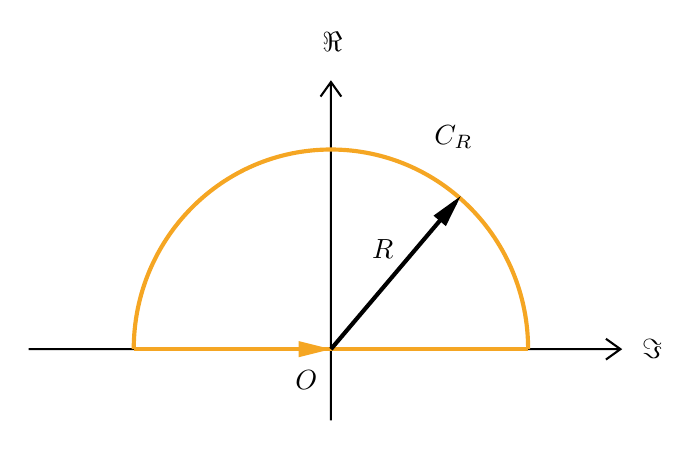
\begin{tikzpicture}[x=0.75pt,y=0.75pt,yscale=-1,xscale=1]
%uncomment if require: \path (0,266); %set diagram left start at 0, and has height of 266

%Shape: Axis 2D [id:dp1282392211894816] 
\draw  (162,181.79) -- (447.09,181.79)(307.61,53.09) -- (307.61,216.09) (440.09,176.79) -- (447.09,181.79) -- (440.09,186.79) (302.61,60.09) -- (307.61,53.09) -- (312.61,60.09)  ;
%Shape: Arc [id:dp1814309272431356] 
\draw  [draw opacity=0][line width=1.5]  (212.6,181.79) .. controls (212.6,181.79) and (212.6,181.79) .. (212.6,181.79) .. controls (212.6,128.66) and (255.14,85.6) .. (307.61,85.6) .. controls (360.08,85.6) and (402.61,128.66) .. (402.61,181.79) -- (307.61,181.79) -- cycle ; \draw  [color={rgb, 255:red, 245; green, 166; blue, 35 }  ,draw opacity=1 ][line width=1.5]  (212.6,181.79) .. controls (212.6,181.79) and (212.6,181.79) .. (212.6,181.79) .. controls (212.6,128.66) and (255.14,85.6) .. (307.61,85.6) .. controls (360.08,85.6) and (402.61,128.66) .. (402.61,181.79) ;  
%Straight Lines [id:da15038694853465828] 
\draw [color={rgb, 255:red, 245; green, 166; blue, 35 }  ,draw opacity=1 ][line width=1.5]    (212.6,181.79) -- (402.61,181.79) ;
\draw [shift={(307.61,181.79)}, rotate = 180] [fill={rgb, 255:red, 245; green, 166; blue, 35 }  ,fill opacity=1 ][line width=0.08]  [draw opacity=0] (15.6,-3.9) -- (0,0) -- (15.6,3.9) -- cycle    ;
%Straight Lines [id:da12449754393780421] 
\draw [color={rgb, 255:red, 0; green, 0; blue, 0 }  ,draw opacity=1 ][line width=1.5]    (307.61,181.79) -- (352.62,128.69) -- (367.5,111.14) ;
\draw [shift={(370.09,108.09)}, rotate = 130.29] [fill={rgb, 255:red, 0; green, 0; blue, 0 }  ,fill opacity=1 ][line width=0.08]  [draw opacity=0] (15.6,-3.9) -- (0,0) -- (15.6,3.9) -- cycle    ;


% Text Node
\draw (289,190.4) node [anchor=north west][inner sep=0.75pt]    {$O$};
% Text Node
\draw (302,27.4) node [anchor=north west][inner sep=0.75pt]    {$\Re $};
% Text Node
\draw (456,175.4) node [anchor=north west][inner sep=0.75pt]    {$\Im $};
% Text Node
\draw (326,127.4) node [anchor=north west][inner sep=0.75pt]    {$R$};
% Text Node
\draw (356,72.4) node [anchor=north west][inner sep=0.75pt]    {$C_{R}$};

% \draw   (239.6, 212.79) circle [x radius= 5, y radius= 5]  (234.6,212.79) -- (244.6,212.79)(239.6,207.79) -- (239.6,217.79) ;
% \draw   (334.61, 116.6) circle [x radius= 5, y radius= 5]  (329.61,116.6) -- (339.61,116.6)(334.61,111.6) -- (334.61,121.6) ;
% \draw   (429.61, 212.79) circle [x radius= 5, y radius= 5]  (424.61,212.79) -- (434.61,212.79)(429.61,207.79) -- (429.61,217.79) ;
% \draw   (396.48, 139.8) circle [x radius= 5, y radius= 5]  (391.48,139.8) -- (401.48,139.8)(396.48,134.8) -- (396.48,144.8) ;
\end{tikzpicture}

